\documentclass[11pt]{article}
\usepackage[margin=1in]{geometry}
\usepackage{graphicx}
\usepackage[dvipsnames]{xcolor}
\usepackage{listings}

\definecolor{persianred}{rgb}{0.8, 0.2, 0.2}
\definecolor{mediumpersianblue}{rgb}{0.0, 0.4, 0.65}
\definecolor{darklavender}{rgb}{0.45, 0.31, 0.59}
\definecolor{lightcodegray}{rgb}{0.97, 0.97, 0.97}
\definecolor{softborder}{gray}{0.8}

\usepackage[colorlinks=true,citecolor=mediumpersianblue,linkcolor=persianred,urlcolor=darklavender]{hyperref}

\lstdefinestyle{pythonstyle}{
    language=Python,
    backgroundcolor=\color{lightcodegray},
    commentstyle=\color{ForestGreen}\itshape,
    keywordstyle=\color{NavyBlue}\bfseries,
    stringstyle=\color{BrickRed},
    basicstyle=\ttfamily\small,
    breaklines=true,
    frame=single,
    framerule=0.3pt,
    rulecolor=\color{softborder},
    numbers=left,
    numbersep=5pt,
}
\lstset{style=pythonstyle}

\title{A Toy Paper for \texttt{matexxe}}
\author{An Example Author}
\date{}

\begin{document}
\maketitle
\tableofcontents
\vspace{1em}

\begin{abstract}
This is a synthetic paper, generated only to demonstrate \texttt{matexxe}'s
project-wide restyling on a document with several figures, each plotted
with a different, mismatched colour scheme -- the kind of inconsistency
that accumulates naturally across a real paper's revision history, as
different co-authors add figures with whatever colour scheme their own
plotting habits default to. None of the numbers below mean anything; only
the colours, and how \texttt{matexxe} reassigns them, do. Every figure's
caption names exactly which colour source it used, linked, so you can look
it up and compare it against whatever \texttt{matexxe} decided to do with
it.
\end{abstract}

\section{Introduction}
\texttt{matexxe} recolours the figures of a paper -- and, when given the
project's own \LaTeX{} source rather than just the compiled PDF, its
hyperlink colours and code-listing syntax highlighting too -- onto a
consistent palette (see \url{https://github.com/MatteoRobbiati/matexxe}).
It decides how many independent colours a document really uses by
clustering hues, then assigns each one a distinct replacement from the
target palette whenever the palette has enough hue families to offer one.
Sections~\ref{sec:categorical} and~\ref{sec:continuous} below run through
the two kinds of figure it treats differently: a handful of discrete
series colours, versus a genuinely continuous colormap encoding a
continuous quantity.

\section{Discrete, categorical figures}
\label{sec:categorical}
The four figures in this section each use a small number of distinct,
named colours -- exactly the case \texttt{matexxe.fit()} is built around.
Figure~\ref{fig:runtime} uses matplotlib's default qualitative cycle,
\href{https://matplotlib.org/stable/users/prev_whats_new/dflt_style_changes.html#colors-in-default-property-cycle}{tab10}.
Figure~\ref{fig:scatter} uses seaborn's
\href{https://seaborn.pydata.org/tutorial/color_palettes.html}{Set2}.
Figure~\ref{fig:convergence} uses matplotlib's
\href{https://matplotlib.org/stable/users/explain/colors/colormaps.html\#qualitative}{Dark2}.
Figure~\ref{fig:donut} uses matplotlib's
\href{https://matplotlib.org/stable/users/explain/colors/colormaps.html\#qualitative}{Accent}.
None of these four sources were designed with one another in mind, which
is exactly the point: a real paper accretes exactly this kind of mismatch
one figure at a time.

\begin{figure}[h]
    \centering
    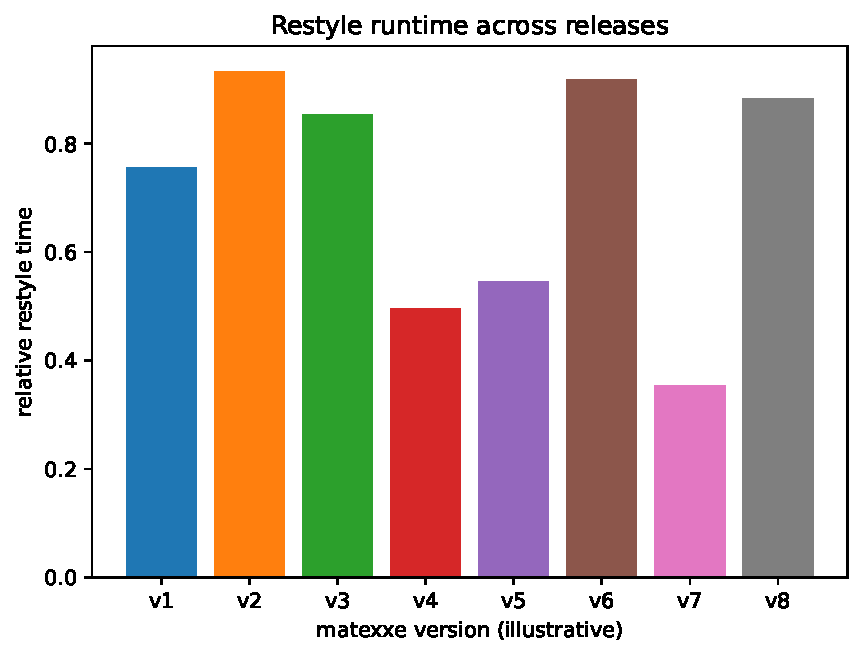
\includegraphics[width=0.85\linewidth]{figures/benchmark_runtime.pdf}
    \caption{Restyle runtime across releases (illustrative numbers). Colour source: matplotlib \href{https://matplotlib.org/stable/users/prev_whats_new/dflt_style_changes.html\#colors-in-default-property-cycle}{tab10}.}
    \label{fig:runtime}
\end{figure}

\begin{figure}[h]
    \centering
    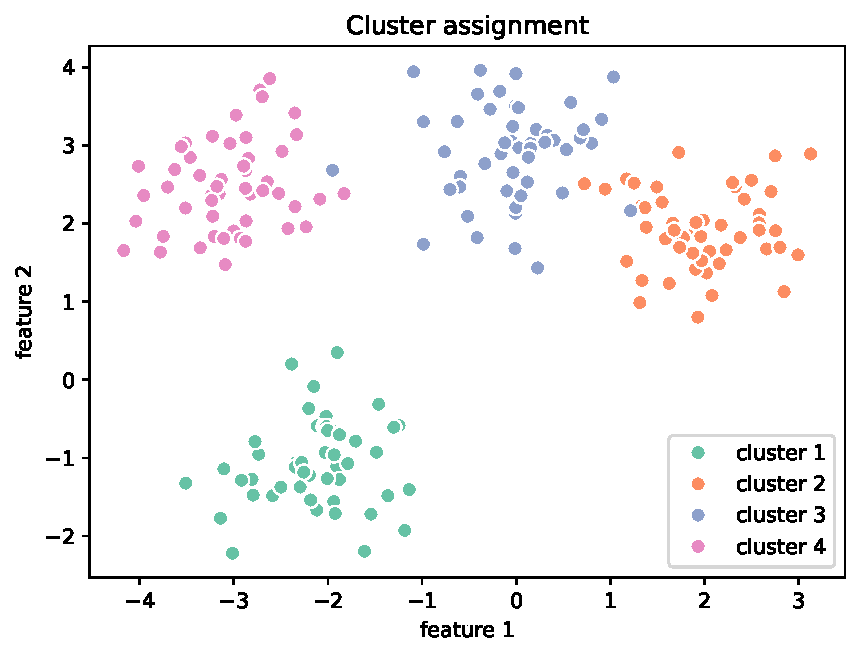
\includegraphics[width=0.85\linewidth]{figures/cluster_scatter.pdf}
    \caption{Cluster assignment in a toy feature space. Colour source: seaborn \href{https://seaborn.pydata.org/tutorial/color_palettes.html}{Set2}.}
    \label{fig:scatter}
\end{figure}

\begin{figure}[h]
    \centering
    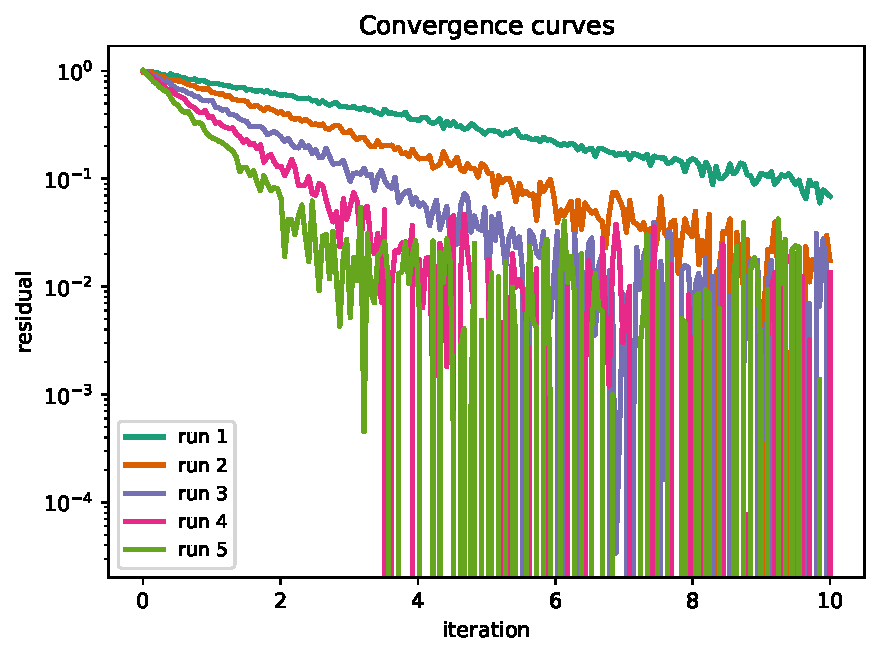
\includegraphics[width=0.85\linewidth]{figures/convergence_curves.pdf}
    \caption{Convergence curves for five synthetic runs. Colour source: matplotlib \href{https://matplotlib.org/stable/users/explain/colors/colormaps.html\#qualitative}{Dark2}.}
    \label{fig:convergence}
\end{figure}

\begin{figure}[h]
    \centering
    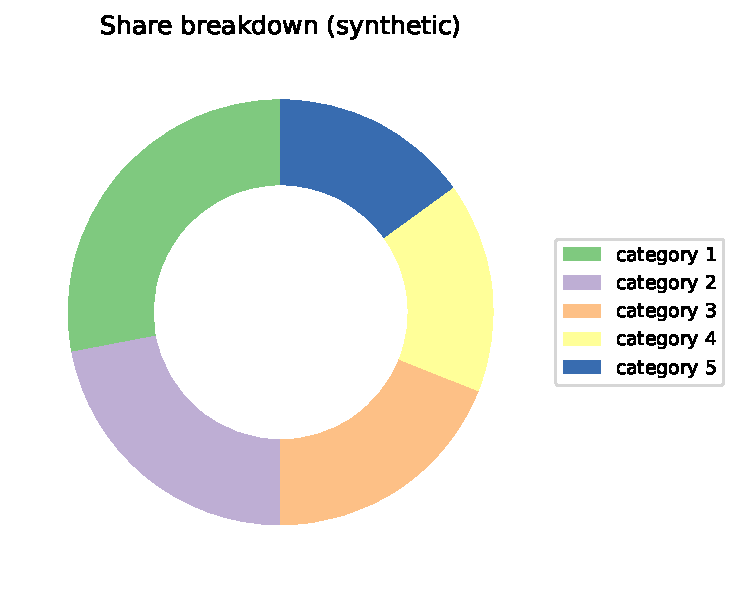
\includegraphics[width=0.7\linewidth]{figures/share_donut.pdf}
    \caption{A synthetic share breakdown. Colour source: matplotlib \href{https://matplotlib.org/stable/users/explain/colors/colormaps.html\#qualitative}{Accent}.}
    \label{fig:donut}
\end{figure}

\clearpage
\section{Continuous colormaps}
\label{sec:continuous}
Not every figure uses a handful of discrete colours. The three figures
below use unrelated \emph{continuous} colormaps: a diverging one, and two
sequential ones with entirely different hues. \texttt{matexxe} recognises
this (see \texttt{matexxe.cluster.looks\_continuous}) and switches to
\texttt{matexxe.fit\_colormap}, which finds each figure's own one or two
dominant hues and blends continuously between their replacements, instead
of snapping a smooth gradient onto a handful of discrete colours and
introducing visible banding.

\begin{figure}[h]
    \centering
    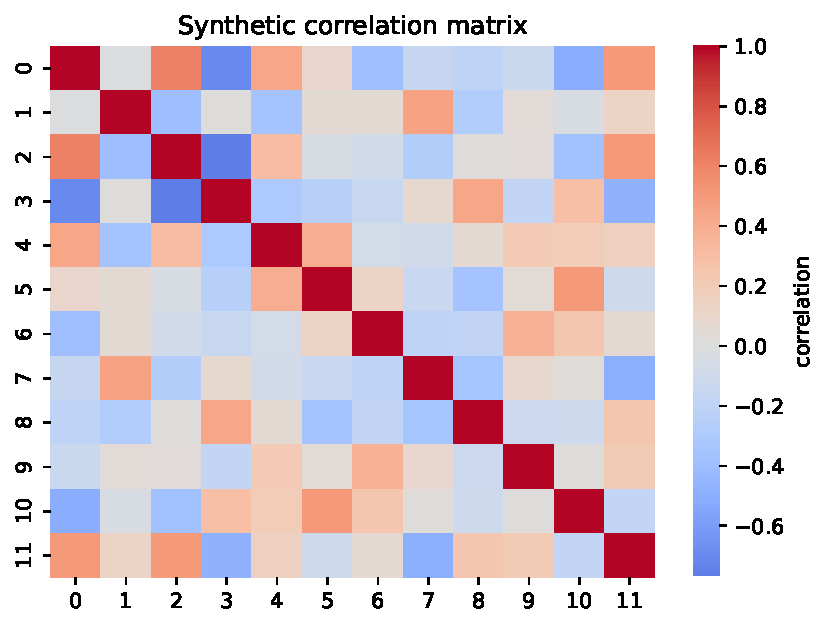
\includegraphics[width=0.75\linewidth]{figures/correlation_heatmap.pdf}
    \caption{A synthetic correlation matrix. Colour source: matplotlib/seaborn \href{https://matplotlib.org/stable/users/explain/colors/colormaps.html\#diverging}{coolwarm} (diverging).}
    \label{fig:heatmap}
\end{figure}

\begin{figure}[h]
    \centering
    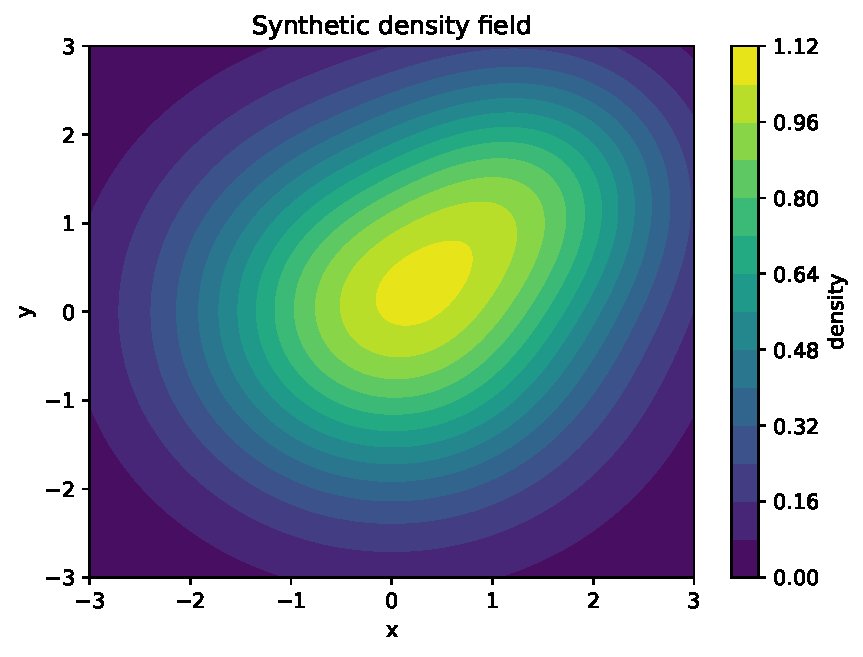
\includegraphics[width=0.75\linewidth]{figures/density_contour.pdf}
    \caption{A synthetic density field. Colour source: matplotlib \href{https://matplotlib.org/stable/users/explain/colors/colormaps.html\#sequential}{viridis} (sequential).}
    \label{fig:contour}
\end{figure}

\begin{figure}[h]
    \centering
    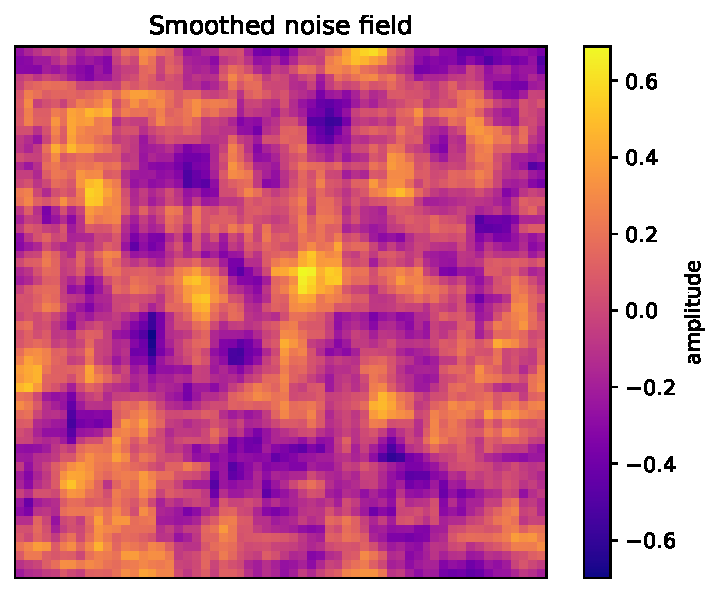
\includegraphics[width=0.75\linewidth]{figures/noise_field.pdf}
    \caption{A smoothed noise field. Colour source: matplotlib \href{https://matplotlib.org/stable/users/explain/colors/colormaps.html\#sequential}{plasma} (sequential, unrelated hue to viridis).}
    \label{fig:noise}
\end{figure}

\clearpage
\section{A raster logo}
\texttt{matexxe} works on plain images too, not just figures inside a
paper. Figure~\ref{fig:jolly} is a flat PNG, included here to exercise that
same path from inside a full project restyle. Its own colours (a
particular yellow and red) happen to already sit close to some palettes'
own yellow and red, so a restyle onto one of those can look almost
unchanged at a glance -- that is \texttt{mode="hue"} correctly doing very
little when there is very little to do, not a sign that nothing happened;
a palette with unrelated hues (e.g. \texttt{violet}) changes it clearly.

\begin{figure}[h]
    \centering
    
\includegraphics[width=0.35\linewidth]{figures/jolly.png}
    \caption{A raster logo, recoloured alongside everything else. Original colours: flat yellow and red, no particular named source.}
    \label{fig:jolly}
\end{figure}

\clearpage
\section{Using matexxe}
Restyling the compiled PDF alone reaches only what ended up embedded as a
drawing object:

\begin{lstlisting}
import matexxe

palette = matexxe.Palette.load("okabe-ito")
paper = matexxe.Painter("main.pdf")
fitted = matexxe.fit(paper, palette)
paper.restyle(fitted, mode="hue")
paper.save("main_restyled.pdf")
\end{lstlisting}

Working from the project's own source, as this paper does, also reaches
hyperlink colours and code-listing syntax highlighting:

\begin{lstlisting}
import matexxe

palette = matexxe.Palette.load("persian")
project = matexxe.Project("toy_paper.zip")
fitted = matexxe.fit(project, palette)
project.restyle(fitted, mode="hue")
project.save("toy_paper_restyled.zip")
\end{lstlisting}

See \url{https://github.com/MatteoRobbiati/matexxe} for the full API.

\section{Conclusion}
This document exists only to be recoloured.

\end{document}
